\section{运动学\quad\tiny 11.2-11.8}
\lsn{1}根据\(v - t\)图像得出匀变速直线运动的公式（至少7个）：

\begin{tikzpicture}[>=stealth,font=\footnotesize]
    \draw[|<->|,thin,gray] (3.25,2.5)--node[fill=white]{ \(\Delta v\)}(3.25,1);
    \filldraw[pattern=north east lines,draw=white,pattern color=red!30] (0,1)--(3,2.5)--(3,1)--(0,1);
    \filldraw[pattern=north west lines,draw=white,pattern color=red!30] (0,0) rectangle(3,1);
    \draw[->,blue] (0,0)--(5,0)node[below]{ \(t\)};
    \draw[->,blue] (0,0)node[below left]{\(O\)}--(0,4)node[right]{ \(v\)};
    \draw[magenta] (0,1)--(4,3)node[below right,black]{ \(a\)};
    \draw[dashed,cyan] (0,2.5)--(3,2.5)--(3,0) (0,1)--(3,1) (0,1.75)--(1.5,1.75)--(1.5,0);
    \node[blue] at(0,1)[left]{ \(v_0\)};
    \node[blue] at(0,2.5)[left]{ \(v_t\)};
    \node[blue] at(3,0)[below]{ \(t\)};
    \node[blue] at(0,1.75)[left]{ \(\overline{v}\)};
    \node[blue] at(1.5,0)[below]{\(\sfrac{t}{2}\)};
    \draw[|<->|,gray,thin] (0,-.8)--node[fill=white]{ \(\Delta t\)}(3,-.8);
  \end{tikzpicture}
\vspace*{2cm}

\lsn{2}写出初速度为0的匀加速直线运动的六个比例关系



\vspace*{5cm}
\lsn{3}在表中填出各个图像中不同元素的物理含义，没有物理意义的画横线

\begin{table}[htbp]
  \begin{tabular}{l|c|c|c}
    \hline
    &\(x -t\)图像&\(v - t\)图像&\(a - t\)图像\\
    \hline
    斜率&&&\\
    \hline
    面积&\tikz \draw (0,.2)--(2,-.2);&&\\
    \hline
    交点&&&\tikz \draw (0,.2)--(2,-.2);\\
    \hline
    零点&&&\tikz \draw (0,.2)--(2,-.2);\\
    \hline
    拐点&&&\tikz \draw (0,.2)--(2,-.2);\\
    \hline
  \end{tabular}
\end{table}

\lsn{4}使用逐差法计算加速度的优点是什么？并推导三个逐差法的公式

\newpage
\lsn{5}表示出下列图像中运动的初速度\(v_0\)与加速度\(a\)，并给出过程

\begin{tikzpicture}[>=stealth,font=\footnotesize]
  \draw[->,blue] (0,0)node[below left]{\(O\)}--(4,0)node[below]{\(t\)};
  \draw[->,blue] (0,0)--(0,3)node[right]{\(\overline{v}\)};
  \draw[magenta] (0,.8)node[left,blue]{\(b\)}--(3,2.5)node[below,blue]{\(k\)};
  \begin{scope}[xshift=5cm]
    \draw[->,blue] (0,0)node[below left]{\(O\)}--(4,0)node[below]{\(\frac{1}{t}\)};
  \draw[->,blue] (0,0)--(0,3)node[right]{\(\frac{x}{t^2}\)};
  \draw[magenta] (0,.8)node[left,blue]{\(b\)}--(3,2.5)node[below,blue]{\(k\)};
  \end{scope}
  \begin{scope}[xshift=10cm]
    \draw[->,blue] (0,0)node[below left]{\(O\)}--(4,0)node[below]{\(x\)};
  \draw[->,blue] (0,0)--(0,3)node[right]{\(v^2\)};
  \draw[magenta] (0,.8)node[left,blue]{\(b\)}--(3,2.5)node[below,blue]{\(k\)};
  \end{scope}
\end{tikzpicture}

\vspace*{3cm}
\lsn{6}\(A\)、\(B\)两辆车（可视为质点）在一条直线上同向运动，\(A\)在\(B\)的正前方\(x_0\)处，它们的\(v - t\)图像如图所示，分析下列情况\(A\)、\(B\)是否相遇，相遇几次

\begin{tikzpicture}[>=stealth,font=\scriptsize]
  \draw[->,blue] (0,0)node[below left]{\(O\)}--(4,0)node[below]{\(t\)};
  \filldraw[pattern=north east lines,draw=white,pattern color=red!30] (0,.5)--(1.5,1.5)--(0,2);
  \draw[->,blue] (0,0)--(0,3)node[right]{\(v\)};
  \draw[magenta] (0,.5)--(3,2.5)node[right]{\(A\)};
  \draw[teal] (0,2)--(3,1)node[right]{\(B\)};
  \node at(.45,1.3){\(\Delta x\)};
\end{tikzpicture}
\begin{itemize}
  \item \(x_0 > \Delta x\)：
  \item \(x_0 = \Delta x\)：
  \item \(x_0 < \Delta x\)：
\end{itemize}

\lsn{7}某同学在实验中得到如下图所示的纸带，其中两点间有4个点未画出，计算并填空（保留三位有效数字）

\begin{tikzpicture}
		\coordinate (o) at(0,0);
		
		\foreach \x/\n in {0/0,.6/1,1.6/2,3/3,4.8/4,7/5,9.6/6}{
			\coordinate (\n) at(\x,0);
			\fill (\n)node[above]{\scriptsize \(\n\)} circle(.03);}
		\foreach \y/\x/\n in {-.7/.6/5.00,-1.1/1.6/11.96,-1.5/3/20.96,-1.9/4.8/31.83,-2.3/7/44.70,-2.7/9.6/76.39}
			\draw[stealth-stealth,thin] (0,\y)--node[fill=white]{\scriptsize \(\n\)}(\x,\y);
		\foreach \x/\y in {0/-2.8,.6/-.8,1.6/-1.2,3/-1.6,4.8/-2.0,7/-2.4,9.6/-2.8}
			\draw[gray] (\x,-.1)--(\x,\y);
    \draw ($(o)+(-.3,.5)$)--++(10.2,0) ($(o)+(-.3,-.5)$)--++(10.2,0)coordinate(a) ($(o)+(-.3,.5)$)--++(-.1,-.1)--++(.2,-.7)--++(-.1,-.2) (a)--++(.1,.1)--++(-.2,.7)--++(.1,.2);
    \node at($(a)+(-.7,1.2)$){\scriptsize 单位：\,\qty{}{cm}};
	\end{tikzpicture}%%始.6,差.4

\vspace*{.5cm}
\(v_1 =\)\lunl{3cm}\qquad \(v_4 =\)\lunl{3cm}

\vspace*{.5cm}
\(a =\)\lunl{3cm}\qquad \(v_0 =\)\lunl{3cm}

\newpage
\lsn{8}\icode{N18Z-MK-SI-L2-260625-001}
\nceeID[3]{2018浙江}{10}
竖直井中的升降机可将地下深处的矿石快速运送到地面。某一竖井的深度约为\qty{104}{m}，升降机运行的最大速度为\qty{8}{m/s}，加速度大小不超过\qty{1}{m/s}，假定升降机到井口的速度为零，则将矿石从井底提升到井口的最短时间是\paren[C]
\begin{choices}
    \item \qty{13}{s}
    \item \qty{16}{s}
    \item \qty{21}{s}
    \item \qty{26}{s}
\end{choices}
\begin{answer}
    C\qquad 提示：升降机先以最大加速度加速至最大速度，匀速运动一段时间后再匀减速，恰好到井口速度为零，时间最短
\end{answer}

\lsn{9}\icode{N18Q-MK-SI-L2-260929-002}
\nceeID[4]{2018海南}{1}
一攀岩者以 \qty{1}{m/s} 的速度匀速向上攀登，途中碰落了岩壁上的石块，石块自由下落。\qty{3}{s} 后攀岩者听到石块落地的声音，此时他离地面的高度约为\paren[C]
\begin{choices}
    \item \qty{10}{m}
    \item \qty{30}{m}
    \item \qty{50}{m}
    \item \qty{70}{m}
\end{choices}
\begin{answer}
    C
\end{answer}

\lsn{10}\icode{N15L-MK-SI-L3-260929-001}
\nceeID[6]{2015山东}{14}
 距地面高 \qty{5}{m} 的水平直轨道上 \(A\)、\(B\) 两点相距 \qty{2}{m}，在 \(B\) 点用细线悬挂一小球，离地高度为 \(h\)，如图。小车始终以 \qty{4}{m/s} 的速度沿轨道匀速运动，经过 \(A\) 点时将随车携带的小球由轨道高度自由卸下，小车运动至 \(B\) 点时细线被轧断，最后两球同时落地。不计空气阻力，取重力加速度的大小 \(g = \qty{10}{m/s^2}\)。可求得 \(h\) 等于\paren[A]

\begin{tikzpicture}[>=stealth,font=\scriptsize]
    \draw[thick] (0,1)--++(4,0) (0,3)--++(4,0);
    \draw[thick, fill=black] (0.15, 3.1) circle (0.1) (.45, 3.1) circle (0.1);
    \draw[thick, fill=gray!30] (0, 3.15) rectangle (.6, 3.5);
    \draw[->] (0,3.7)--(.6,3.7); 
    \coordinate (A) at (2.2, 3);
    \coordinate (B) at (3.4, 3);
    \node[above] at (A) {\(A\)};
    \node[above] at (B) {\(B\)};
    \draw[thick, fill=gray!50] ($(A)+(0,-.1)$) circle (0.1); 
    \draw[purple] (B)--(3.4, 2.5);
    \draw[dashed,cyan] (3.1,2.4)--++(.7,0);
    \draw[fill=gray!50] (3.4, 2.5) circle (0.1);
    \draw[<->] (3.6, 1) -- (3.6, 2.4) node[midway, right] {\(h\)};
\end{tikzpicture}
\begin{choices}
    \item \qty{1.25}{m}
    \item \qty{2.25}{m}
    \item \qty{3.75}{m}
    \item \qty{4.75}{m}
\end{choices}
\begin{answer}
    A\qquad 提示：\(A\)处小球\qty{1}{s}落地，小车由\(A\) 到\(B\) 经过\qty{0.5}{s}，可知\(B\) 处小球下落\qty{0.5}{s}
\end{answer}



\lsn{11}\icode{N23L-MK-SI-L3-261001-002}
\nceeID[4]{2023山东}{6}
如图所示，电动公交车做匀减速直线运动进站，连续经过\(R\)、\(S\)、\(T\)三点，已知\(ST\)间的距离是\(RS\)间的两倍，\(RS\)段的平均速度是\qty{10}{m/s}，\(ST\)段的平均速度是\qty{5}{m/s}，则公交车经过\(T\)点时的瞬时速度是\paren[C]

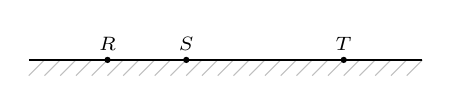
\begin{tikzpicture}[font=\scriptsize]
    \foreach \x in {-1,-.8,...,3.8}
        \draw[gray!50] (\x,-.2)--++(.2,.2);
    \draw[thick] (-1,0)--(4,0);
    \foreach \x/\str in{0/R,1/S,3/T}
        \fill (\x,0)node[above]{\(\str\)} circle(.04);
\end{tikzpicture}
\begin{choices}
    \item \qty{3}{m/s}
    \item \qty{2}{m/s}
    \item \qty{1}{m/s}
    \item \qty{0.5}{m/s}
\end{choices}
\begin{answer}
    C\qquad 提示：由两段位移与平均速度关系可知，若\(RS\)用时为\(\tau \)，则\(ST\)用时为\(4\tau\)

    \begin{tikzpicture}[>=stealth,font=\scriptsize]
        \draw[->,blue] (0,0)node[below left]{\(O\)}--(5,0)node[below]{\(t\)};
        \draw[->,blue] (0,0)--(0,4)node[right]{\(v\)/(\qty{}{m\cdot s^{-1}})};
        \draw[dashed,cyan] (0,3)node[blue,left]{10}--(.4,3)--(.4,0) (0,1.5)node[blue,left]{5}--(2.4,1.5)--(2.4,0)node[blue,below]{\(3\tau\)} (0,.3)--(4,.3)--(4,0)node[blue,below]{\(5\tau\)} (.8,2.7)--(.8,0)node[blue,below]{\(\tau\)};
        \draw[purple] (0,3.3)--(4,.3);
    \end{tikzpicture}
\end{answer}

\lsn{12}\icode{E-MK-MU-L2-260928-001}
（多选）
某物体做直线运动的 \(\frac{x}{t}-t\) 图像如图所示。下列说法正确的是\paren[AD]

\begin{tikzpicture}[>=stealth,font=\scriptsize]
	\draw[->,blue] (0,0)node[left]{\(0\)}--(3.5,0)node[below]{\(t\)/\qty{}{s}};
	\draw[->,blue] (0,-1)--(0,2.5)node[right]{\(\frac{x}{t}\)/(\qty{}{m\cdot s^{-1}})};
	\draw[dashed,cyan] (0,1)--(1.5,1)--(1.5,0);
	\draw[magenta] (0,-.5)--(2.6,2.1);
	\foreach \x/\n in {.5/1,1.5/3,3/6}
		\draw[blue] (\x,.1)--(\x,0)node[below]{\(\n\)};
	\foreach \y/\n in {1/10,2/20}
		\draw[blue] (0,\y)node[left]{\(\n\)}--++(.1,0);
\end{tikzpicture}
\begin{choices}
	\item 物体的加速度大小为\qty{10}{m/s^2}
	\item 物体的初速度大小为\qty{10}{m/s}
	\item \qty{1}{s}时，物体的速度大小为\qty{10}{m/s}
	\item 在 \(0 \sim 3\) \qty{}{s}内，物体的位移大小为\qty{30}{m}
\end{choices}
\begin{answer}
	AD\qquad 提示：\(\frac{x}{t} = \frac{a}{2}\cdot t + v_0\)
\end{answer}

\lsn{13}\icode{E-MK-SI-L2-260928-001}
一个朝着某方向做直线运动的物体，在时间\(t\)内的平均速度是\(v\)，紧接着在时间\(\frac{t}{2}\)内的平均速度是\(\frac{v}{2}\)，则物体在这段时间内的平均速度是\paren[D]
\begin{choices}
	\item \(v\)
	\item \(\dfrac{2}{3}v\)
	\item \(\dfrac{4}{3}v\)
	\item \(\dfrac{5}{6}v\)
\end{choices}
\begin{answer}
	D\qquad \kaishu 由平均速度的定义可知\(\overline{v} = \frac{vt + \frac{v}{2}\cdot\frac{t}{2}}{t + \frac{t}{2}} = \frac{5}{6}v\)
\end{answer}

\lsn{14}\icode{E-MK-SI-L2-260928-003}
\(A\)、\(B\) 两辆汽车同时从坐标原点沿同一方向做直线运动，\(A\) 车做刹车运动，它们速度的平方 \( v^2 \) 随位置 \( x \) 变化的图像如图所示，分别对应直线 \(A\) 和直线 \(B\)，以两车运动方向为正方向，下列说法正确的是\paren[C]

\begin{tikzpicture}[>=stealth,font=\scriptsize]
	\draw[->,blue] (0,0)node[below left]{0}--(4,0)node[below]{\(x\)/\qty{}{m}};
	\draw[->,blue] (0,0)--(0,3)node[right]{\(v^2\)/ (\qty{}{m^2\cdot s^{-2}})};
	\draw[dashed,cyan] (0,1.3)--(3,1.3)--(3,0) (2,{2.6/3})--(2,0);
	\draw[magenta] (0,2.6)--(3,0);
	\draw[teal] (0,0)--(3.5,{3.5*1.3/3});
	\foreach \x/\c in {1/3,2/6,3/9}
		\draw[blue] (\x,.1)--(\x,0)node[below]{\(\c\)};
	\foreach \y/\c in {1.3/18,2.6/36}
		\draw[blue] (.1,\y)--(0,\y)node[left]{\(\c\)};
\end{tikzpicture}
\begin{choices}
	\item 汽车 \(A\) 的加速度为\qty{2}{m/s^2}
	\item 汽车 \(B\) 的加速度为\qty{2}{m/s^2}
	\item 汽车 \(A\) 在\(0\sim 4\)\qty{}{s} 内的位移大小为\qty{9}{m}
	\item 汽车 \(A\)、\(B\) 在 \( x= \)\qty{6}{m} 处相遇
\end{choices}
\begin{answer}
	C\quad 提示：注意两车初始位置，由\(v^2 - v_0^2 = 2ax\)可知\(v^2 = 2a\cdot x + v_0^2\)
\end{answer}

\lsn{15}\icode{E-MK-CA-L3-260929-001}
在某次班级活动中，甲同学在前，乙同学在后，两者静止且相距 \(x_0 =\)\qty{4.5}{m}，甲到终点的距离 \(L =\)\qty{40}{m}，甲以 \(a_1 =\) \,\qty{2}{m/s^2}的加速度由静止开始匀加速跑向终点，在甲出发 \(t_0 =\) \,\qty{2}{s}后，乙以 \(a_2 =\) \,\qty{3}{m/s^2}的加速度由静止开始匀加速追甲。已知甲、乙能达到的最大速度分别为 \(v_{m1} =\) \,\qty{6}{m/s}和 \(v_{m2} =\) \,\qty{9}{m/s}，两者达到最大速度后均做匀速运动。
\begin{enumerate}
	\item 求两者的最大距离 \(x_{\max}\);
	\item 试通过计算判断乙能否在终点前追上甲。
\end{enumerate}
